%%%%%%%%%%%%%%%%%%%%%%%%%%%%%%%%%%%%%%%%%%%%%%%%%%%%%%%%%%%%%%%%%%%%%%%%%%%%%%%%%%%%%%%%%%%
% LaTeX Template of the Chair of Enterprise Systems
% Version 0.91
% Author: Markus Dietsche
% Questions? Feedback? Remarks? -> dietsche.markus@gmail.com
%%%%%%%%%%%%%%%%%%%%%%%%%%%%%%%%%%%%%%%%%%%%%%%%%%%%%%%%%%%%%%%%%%%%%%%%%%%%%%%%%%%%%%%%%%%

%%%%%%%%%%%%%%%%%%%%%%%%%%%%%%%%%%%%%%%%%%%%%%%%%%%%%%%%%%%%%%%%%%%%%%%%%%%%%%%%%%%%%%%%%%%
% !!! IMPORTANT !!!
% 1) Use/upload whole template folder, including "fonts" and "images" subfolder
%    e.g Overleaf: "upload" (top-left) -> Select all contents of template folder
% 2) Make sure XeLaTeX is selected as Latex Compiler 
%    e.g Overleaf: "Menu" (top-left) -> Compiler -> Select "XeLaTeX"
% 3) Make sure 
%    e.g Overleaf: "Menu" (top-left) -> Main document -> Select "main.tex
%%%%%%%%%%%%%%%%%%%%%%%%%%%%%%%%%%%%%%%%%%%%%%%%%%%%%%%%%%%%%%%%%%%%%%%%%%%%%%%%%%%%%%%%%%%

%%%%%%%%%%%%%%%%%%%%%%%%%%%%%%%%%%%%%%%%%%%%%%%%%%%%%%%%%%%%%%%%%%%%%%%%%%%%%%%%%%%%%%%%%%%
% Changelog
% 0.91 Switched bibliography backend from biber to bibtex (Thanks to Fareed! :-)
%%%%%%%%%%%%%%%%%%%%%%%%%%%%%%%%%%%%%%%%%%%%%%%%%%%%%%%%%%%%%%%%%%%%%%%%%%%%%%%%%%%%%%%%%%%


%%%%%%%%%%%%%%%%%%%%%%%%%%%%%%%%%%%%%%%%%%%%%%%%%%%%%%%%%%%%%%%%%%%%%%%%%%%%%%%%%%%%%%%%%%%
% Settings for LaTeX Template of the Chair of Enterprise Systems
% Version 0.91
% Author: Markus Dietsche
% Questions? Feedback? Remarks? -> dietsche.markus@gmail.com
%%%%%%%%%%%%%%%%%%%%%%%%%%%%%%%%%%%%%%%%%%%%%%%%%%%%%%%%%%%%%%%%%%%%%%%%%%%%%%%%%%%%%%%%%%%

%%%%%%%%%%%%%%%%%%%%%%%%%%%%%%%%%%%%%%%%%%%%%%%%%%%%%%%%%%%%%%%%%%%%%%%%%%%%%%%%%%%%%%%%%%%
% Document settings (DO NOT CHANGE) -> go to "Title Page" 
%%%%%%%%%%%%%%%%%%%%%%%%%%%%%%%%%%%%%%%%%%%%%%%%%%%%%%%%%%%%%%%%%%%%%%%%%%%%%%%%%%%%%%%%%%%

\documentclass[12pt]{article}
\usepackage[utf8]{inputenc}
\usepackage{fontspec}
 % Times New Roman
\setmainfont[Path = ./fonts/,
BoldFont=timesbd.ttf,
ItalicFont=timesi.ttf,
BoldItalicFont=timesbi.ttf
]{times.ttf}
 
% include graphics, set path to folder containing images
\usepackage{graphicx}
\graphicspath{ {./images/} } 
\usepackage{setspace}

% Table spacing and wrappings
\usepackage{array}
\setlength\extrarowheight{5pt}

% Long Tables
\usepackage{longtable}

% PDFs
\usepackage{pdfpages}

% Landscape
\usepackage{lscape} 


\renewcommand{\baselinestretch}{1.5} % set standard text spacing to 1.5

% change separation between dots
\usepackage{tocloft}
% add dots to sections
\renewcommand{\cftsecleader}{\cftdotfill{\cftdotsep}} 
% reduce space in-between dots 
\renewcommand{\cftdotsep}{0} 

% remove page number on ToC
\addtocontents{toc}{\protect\thispagestyle{empty}}

% List of Abbreviations
\usepackage{nomencl}
\makenomenclature

\renewcommand{\nomname}{}
\setlength{\nomitemsep}{8pt}
\usepackage{etoolbox}
\renewcommand\nomgroup[1]{%
  \item[\Large\bfseries{
  \ifstrequal{#1}{A}{List of Abbreviations}{}}%
]\vspace{10pt}}

% margins 
\usepackage[paper=a4paper,margin=4cm]{geometry} % margins for title page

% clickable ToC 
\usepackage{hyperref}
\hypersetup{
    colorlinks,
    citecolor=black,
    filecolor=black,
    linkcolor=black,
    urlcolor=black
}

% unnumbered sections with headings
\newcommand{\sectionunnumbered}[1] {
  \section*{#1} % Section heading, without number
  \addcontentsline{toc}{section}{#1} % Add section heading to ToC
}

% bibliography + MISQ Style
\usepackage[english]{babel}
\usepackage{csquotes}

\usepackage[
  backend=bibtex,
  style=authoryear,
  giveninits=true,
  eprint=false,
  maxbibnames=99,
  maxcitenames=2,
  uniquename=init,
  bibencoding=utf8
]{biblatex}
\addbibresource{bibliography.bib}

\renewcommand*{\newunitpunct}{\addcomma\space}

\DeclareNameAlias{sortname}{family-given}
%\DeclareDelimFormat[bib,biblist]{nametitledelim}{\addperiod\space} % TODO Markus why not required?

\renewcommand*{\intitlepunct}{\addspace}

\renewbibmacro*{volume+number+eid}{%
  \setunit{\addspace}%
  \printtext[parens]{%
    \printfield{volume}%
    \setunit*{\addcolon}%
    \printfield{number}}%
  \setunit{\addcomma\space}%
  \printfield{eid}}

\DeclareFieldFormat{doi}{%
  \mkbibparens{%
    doi\addcolon\space
    \ifhyperref
      {\href{https://doi.org/#1}{\nolinkurl{#1}}}
      {\nolinkurl{#1}}}}

\renewbibmacro*{doi+eprint+url}{%
  \setunit{\addspace}%
  \iftoggle{bbx:doi}
    {\printfield{doi}}
    {}%
  \newunit\newblock
  \iftoggle{bbx:eprint}
    {\usebibmacro{eprint}}
    {}%
  \newunit\newblock
  \iftoggle{bbx:url}
    {\usebibmacro{url+urldate}}
    {}}
    
% date formats
\usepackage{datetime}
\newdateformat{titledate}{\THEDAY. \monthname~\THEYEAR} % format of date on title page. 


% fake small caps
\usepackage{fontspec}
\makeatletter
\newlength\fake@f
\newlength\fake@c
\def\fakesc#1{%
  \begingroup%
  \xdef\fake@name{\csname\curr@fontshape/\f@size\endcsname}%
  \fontsize{\fontdimen8\fake@name}{\baselineskip}\selectfont%
  \uppercase{#1}%
  \endgroup%
}
\makeatother
\newcommand\fauxsc[1]{\fauxschelper#1 \relax\relax}
\def\fauxschelper#1 #2\relax{%
  \fauxschelphelp#1\relax\relax%
  \if\relax#2\relax\else\ \fauxschelper#2\relax\fi%
}
\def\Hscale{.83}\def\Vscale{.72}\def\Cscale{1.00}
\def\fauxschelphelp#1#2\relax{%
  \ifnum`#1>``\ifnum`#1<`\{\scalebox{\Hscale}[\Vscale]{\uppercase{#1}}\else%
    \scalebox{\Cscale}[1]{#1}\fi\else\scalebox{\Cscale}[1]{#1}\fi%
  \ifx\relax#2\relax\else\fauxschelphelp#2\relax\fi}


%%%%%%%%%%%%%%%%%%%%%%%%%%%%%%%%%%%%%%%%%%%%%%%%%%%%%%%%%%%%%%%%%%%%%%%%%%%%%%%%%%%%%%%%%%%
% "Title Page" Section
%%%%%%%%%%%%%%%%%%%%%%%%%%%%%%%%%%%%%%%%%%%%%%%%%%%%%%%%%%%%%%%%%%%%%%%%%%%%%%%%%%%%%%%%%%%

\begin{document}

\begin{titlepage}
	\centering

    
\includegraphics[width=7.38cm]{logo_university_of_mannheim.png}\par

	\vspace{1.25cm}
	{\scshape\Large\uppercase{Design Elements of Digital Nudges and Effects on Consumer Behavior: \\ A Literature Review}\par}
	
	\vspace{2.5cm}
	{\linespread{1}\normalsize Seminar Thesis\\
	 of  \par}
	
	{\large \fauxsc{Marvin Messenzehl}\par}
	
	\vspace{0.5cm}
	{\small \titledate\today \par} % uncomment this line use date of today automatically
% {\small 12. March 2019 \par} %
	
	\vspace{0.3cm}
	{\footnotesize  Matriculation Number\\
	1585571\par}
	
	\vspace{2.5cm}
	\hrulefill\\	
	\vspace{1.0cm}
	{\linespread{1}\normalsize Submitted at the Chair of Enterprise Systems\\
	University of Mannheim\par}
	
	\vspace{0.3cm}
	{\linespread{1}\normalsize  Reviewer: Prof. Dr. Hartmut Höhle\\
	Supervisor: Florian Pethig\par}


\end{titlepage}
\renewcommand{\contentsname}{Table of Contents} % table of content heading



%%%%%%%%%%%%%%%%%%%%%%%%%%%%%%%%%%%%%%%%%%%%%%%%%%%%%%%%%%%%%%%%%%%%%%%%%%%%%%%%%%%%%%%%%%%
% "Table of Content", "List of Figures", "List of Tables" Section
\newgeometry{top=3cm,bottom=2cm,right=3cm,left=3cm} % update page margins
%%%%%%%%%%%%%%%%%%%%%%%%%%%%%%%%%%%%%%%%%%%%%%%%%%%%%%%%%%%%%%%%%%%%%%%%%%%%%%%%%%%%%%%%%%%

\pagenumbering{roman} % set capital roman page numbers: I, II, ...
\clearpage \setcounter{page}{2} % count cover page
\tableofcontents

\newpage
\addcontentsline{toc}{section}{\listfigurename}
\listoffigures

\newpage
\addcontentsline{toc}{section}{\listtablename}
\listoftables
\newpage

%%%%%%%%%%%%%%%%%%%%%%%%%%%%%%%%%%%%%%%%%%%%%%%%%%%%%%%%%%%%%%%%%%%%%%%%%%%%%%%%%%%%%%%%%%%
% "Abbreviations" Section 
%%%%%%%%%%%%%%%%%%%%%%%%%%%%%%%%%%%%%%%%%%%%%%%%%%%%%%%%%%%%%%%%%%%%%%%%%%%%%%%%%%%%%%%%%%%

\nomenclature[A]{\textbf{BI}}{Business Intelligence}
\nomenclature[A]{\textbf{BPI}}{Business Process Intelligence}
\nomenclature[A]{\textbf{BPM}}{Business Process Management}
\nomenclature[A]{\textbf{DW}}{Data Warehouse}
\nomenclature[A]{\textbf{PM}}{Process Mining}
\nomenclature[A]{\textbf{GT}}{Geogria Tech}

\printnomenclature[7cm]
\addcontentsline{toc}{section}{List of Abbreviations}
\newpage

%%%%%%%%%%%%%%%%%%%%%%%%%%%%%%%%%%%%%%%%%%%%%%%%%%%%%%%%%%%%%%%%%%%%%%%%%%%%%%%%%%%%%%%%%%%
% "Abstract" Section
%%%%%%%%%%%%%%%%%%%%%%%%%%%%%%%%%%%%%%%%%%%%%%%%%%%%%%%%%%%%%%%%%%%%%%%%%%%%%%%%%%%%%%%%%%%

\sectionunnumbered{Abstract}
With the release of the book \textit{Nudge}, by Richard Thaler and Cass Sunstein, the concept of nudging began to gain interest in research. Nudging describes a way that alters people's decisions and behaviors predictably. Therefore, this concept has promising benefits for different target groups. On the one hand, a business can increase conversions with precisely designed nudges and on the other hand users face easier decisions they have to make which overall can increase the user experience and customer satisfaction. This paper builds a literature review of different research streams concerning nudges in digital environments. A qualitative representation of the current research in form of academic journal articles is gathered, reviewed and analyzed.
This literature review sees a clear focus of nudging in the application area of consumer choice and has an emphasis on empirical studies. The vast majority of research studies the effect of social, as well as default nudges. To design those nudges, researchers consider only a few specific biases such as the status quo bias and social norms. Overall, current research provides an isolated view on decision-making with the focus on the nudge itself. No research with regards to the overall user experience is identified. The results of this literature review provide essential findings for future research in the area of digital nudging. This paper recommends a focus for future research on complex decision domains like the finance and insurance sector, as well as an extended analysis of other heuristics and biases such as the middle-option bias and scarcity effect. Furthermore, the findings of this paper provide practical insights for product designers and -managers to facilitate decision-making processes in digital applications.

\newpage

%%%%%%%%%%%%%%%%%%%%%%%%%%%%%%%%%%%%%%%%%%%%%%%%%%%%%%%%%%%%%%%%%%%%%%%%%%%%%%%%%%%%%%%%%%%
% "Main Document" Section
\pagenumbering{arabic} % set capital roman page numbers: 1,2,...
%%%%%%%%%%%%%%%%%%%%%%%%%%%%%%%%%%%%%%%%%%%%%%%%%%%%%%%%%%%%%%%%%%%%%%%%%%%%%%%%%%%%%%%%%%%

% Include chapters with the \input command
\newpage
\section{Introduction}
It is a typical Sunday afternoon. John is sitting on the couch, watching a match of his favorite soccer club on TV. On his lap, he is holding his tablet while browsing the internet. John is looking for a good travel deal for his upcoming trip to Bali with his wife. On a news site, a prominent and bright advertisement catches his attention: \textit{Booking.com - From cozy country homes to funky city apartments}. That is precisely what John is looking for. He clicks the link and finds himself on a website full of images of traveling people. Moreover, there is a search field, too. John enters his dream-destination, the travel time and clicks on \textit{search}. After some seconds a list of hotels shows up. The first one catches his eyes. A beautiful beach, a nice pool and cozy, big bedrooms. Perfect. He clicks on the details. However,  John is starting to become nervous. A bright, red piece of information is showing him that this room has been booked three times in the last twelve hours. Also, there are only seven rooms left! His heart beats faster. He needs to get that deal! John clicks on the reservation button. He has just been nudged\footnote{A screenshot of the web page can be found in the appendix on Figure \ref{fig:booking}}.
\\
%In the last ten years, our lives became more and more digitized. We buy products in online shops, book our next trip and holidays on digital hotel platforms and even manage our finances with the help of our smartphones (\cite{schneider_digital_2018}). All those digital environments have one thing in common. Choices. All the time users are faced with choices they have to take,  even if people do not perceive it directly. There a lot of things digital (and also non-digital) environments that frame the whole choice process and therefore influence the decision-making through certain biases and heuristics (\cite{tversky_judgment_1974}). 

"What is chosen often depends upon how the choice is presented" (\cite[p.488]{johnson_beyond_2012}). This presentation describes the term of choice architecture, which should "alter people's behavior in a predictable way" (\cite[p.6]{thaler_nudge:_2009}). In the age of digital transformation, digital environments are powerful tools where the choice architecture can be controlled in detail and therefore provide opportunities to influence user behavior in several ways. This process is called \textit{digital nudging} (\cite{weinmann_digital_2016}).
Digital nudging and the design of online choice architecture have recently gained interest in different research areas. Because of the underlying complexity, it is significant to understand how such nudges influence the decision-making of the user and how the cognitive biases behind this process are working. Especially in consumer choices, there are good and bad patterns of nudging when it comes to an ethical point of view (\cite{sunstein_nudging_2015}). This paper presents a systematic literature review of the last ten years to get a better understanding of how digital nudges influence consumer choice. 
\\

The goals of this paper are two-folded. The primary aim is to provide an overview of different research streams within the topic of digital nudges. The paper focuses here on digital nudges in the area of consumer choice and their specific design elements. Literature in this domain shall be gathered, reviewed and analyzed. Different target groups, such as product designers, managers and user interface designers, can use this knowledge to implement nudges in digital applications more thoughtful and efficient. Furthermore, the correct use of nudges in combination with design elements can increase user experience, customer satisfaction and therefore conversion rates for digital products (\cite{conitzer_hide_2012}).
Secondary, a recommendation for future research is derived from the analysis to advance research in this particular subject. Because of its multidisciplinary nature, research on digital nudges may contribute to several scientific domains, such as information systems, psychology, and behavioral economics.


\newpage
\section{Conceptual Background}

\subsection{ The birth of nudging}
With the release of the book \textit{Nudge} in 2009, Thaler and Sunstein have laid the foundation for the concept of nudging. This concept was primarily a subject of research in behavioral economics. Because of the multifaceted meaning of the word \textit{nudging}, a consistent understanding is essential. This paper uses the central definition of nudges from Thaler and Sunstein (\citeyear[p.6]{thaler_nudge:_2009}): \textit{"A nudge [...] is any aspect of the choice architecture that alters people's behavior in a predictable way without forbidding any options or significantly changing their economic incentives."}
One central aspect of this definition is the economic incentive of the consumer, which should not be changed. This fundamental thought is the basis of a concept called libertarian paternalism (\cite{thaler_nudge:_2009}). In this concept, choices are influenced in a way to make them easy for people and aligning them with their interests. One example of that would be "putting the fruit at eye level" (\cite[p.6]{thaler_nudge:_2009}). However, banning the food would not be a nudge. Since influencing people's behavior can simply be exploited, the ethical viewpoint on nudges should always be kept in mind (\cite{sunstein_nudging_2015}).
\\

Because the human brain only has a limited capacity to store and process information, the consumer often feels subconsciously overloaded. This overloading is called cognitive limitation, which results in greater difficulty and complexity when it comes to decisions and cognitively demanding tasks (\cite{broniarczyk_decision_2014}). Therefore "many decisions are based on beliefs concerning the likelihood of uncertain events" (\cite[p.1124]{tversky_judgment_1974}). Based on this assumption Tversky and Kahneman (\citeyear{tversky_judgment_1974}) formulated three heuristics and several biases that build the foundation of human decision making. Those heuristics and biases act as a psychological guideline in digital nudging. Table \ref{table:schneider} gives an overview of the most used heuristics and biases in nudging.
\\

Besides the cognitive foundation of decision making, there are five general principles of nudging (based on Thaler et al. \citeyear{thaler_choice_2010})
\paragraph{Incentive}
Those kinds of nudges aim to make incentives more salient to increase the effectiveness of the nudge. The focus lays on the motivation behind the decision. The nudge should match the users' motivation. A motivation in nudges goes beyond monetary and material incentives.
\paragraph{Understanding mapping}
Making the consequence of a choice clear is an essential part of easing the decision-making process. Mainly, this concerns complex information that is difficult to evaluate, for example, the number of megapixels of a camera. Frequently, customers cannot evaluate this information directly, based on a single number. A rational mapping could be to display the maximum printable size of a taken picture (\cite{weinmann_digital_2016}). This way, the product attribute can be compared efficiently.
\paragraph{Defaults}
The pre-selection of certain information has an enormous effect. By changing the default option, consumers are more likely to choose an option near to the selected default or even the default itself. One prominent example of such a nudge is the question if people want to consent to be an organ donor. Simply by changing the default option, in this case, can nearly double the percentage of organ donors (\cite{johnson_defaults_2003}). 
\paragraph{Giving feedback}
By giving feedback during the decision-making process, people can evaluate their performance and estimate the output of the decision. Such an example can be found in an experiment for pre-ordering lunch in a school. Students arrange their lunch with different kind of foods. According to this arrangement they receive feedback about how balanced and healthy their food compilation is. Only based on this feedback, students selected significantly more fruits and vegetables in their meals (\cite{miller_effects_2016}).
\paragraph{Expecting error}
Precisely because of the underlying complexity of the decision-making process, it is necessary to expect errors to be made. Such errors should be taken into account when designing a decision, and the environment should be as forgiving as possible. That is why customers first have to remove their credit card from a cash machine before they can obtain the money. In this way, the system makes sure that users do not make serious errors (\cite{weinmann_digital_2016}).
\paragraph{Structure complex choices}
A difficult task in decision-making is to compare different product alternatives. By listing all attributes, people can evaluate trade-offs and make better decisions, based on their interests. In a field experiment, researches evaluated the effect of such a nudge in a bar regarding craft beer choice. By listing more product attributes that naturally describe the taste, people could decide more easily what they want to order (\cite{malone_excessive_2017}).


\subsection{(Online) Choice Architectures}
The concept of nudging builds on the assumption that decisions are made in choice architectures, which are designed by choice architects (\cite{thaler_nudge:_2009}). In this case, the parallel to a "real" architect of a building is not far-fetched. Johnson et al. (\cite{johnson_beyond_2012}) describe the power of such choice architects and how they guide people's choices like other architects guide behavior through the design of the "placement of doors, hallways, staircases, and bathrooms. Just like in a hotel or building, there is no neutral architecture" (\cite[p.488]{johnson_beyond_2012}) for choices. Even small things like a default choice affect decision-making. The mobile payment app Square, for example, nudges people into giving tips only by setting a default value. This way, customers actively must select a \textit{no tipping} option if they do not want to give a tip (\cite{weinmann_digital_2016}). "Because advances in technology and the user of the Internet also provide new ways of finding, creating and exchanging information [...]" (\cite[p.609]{broniarczyk_decision_2014}) people automatically shift a majority of their decisions to the online or digital world. However, digital environments are more complicated. Just like in non-digital environments, there is no neutral way to present choices. Therefore, any user interface can be viewed as a digital choice environment (\cite{schneider_digital_2018}). This ranges from the positioning of elements to the colors in the interface, the language and even the design elements themselves and beyond.
To get a better understanding of how such choice architectures can be built and which elements are available, Münscher et al. (\citeyear{munscher_review_2016}) created a taxonomy of choice architecture categories and their techniques. Overall, there are three major categories with several associated techniques. 
\paragraph{Decision information}
The first level of choice architectures targets the "presentation of decision-relevant information" (\cite[p.514]{munscher_review_2016}). One important aspect is that this category only includes the presentation and no altering of the options itself. Techniques for that choice architecture category are the translation of information, visibility of information and the providence of social reference points.
\paragraph{Decision structure}
Secondly, choice architects directly modify the available options of choice itself. This modification includes techniques like choice defaults, the related effort and consequences of an option and also the range of composition and options.
\paragraph{Decision assistance}
Lastly, choices can be designed in such a way that consumers follow their intentions. Techniques for such assistance can be the fostering of a commitment or by providing reminders of the preferred behavior.

\subsection{Nudging is becoming digital}
Because various choices we take today "involve some form of information technology" (\cite[p.490]{johnson_beyond_2012}), the concept of nudging recently gained interest in research of different disciplines. Thereby, the underlying concepts of non-digital nudges are transferred and adapted in digital environments. According to Weinmann et al.  (\citeyear{weinmann_digital_2016}), digital nudges are defined as follows:
\textit{"Digital nudging is the use of user-interface design elements to guide people's behaviors in digital choice environments"} (\cite[p.433]{weinmann_digital_2016}).
\\

Digital environments face multiple sources of decision difficulty such as task complexity, information load, information uncertainty, conflicts, emotional difficulty and preference uncertainty (\cite{broniarczyk_decision_2014}). To face those challenges, the use of cognitive heuristics and biases can act as a baseline to design digital nudges. Different user-interface design elements induce different nudges. Table \ref{table:schneider} in the appendix gives an overview of the different biases, in which way they influence decision-making and how those are translated to specific design elements.
\\

Even though nudges aim to influence behavior in digital environments, they should not be mistaken with persuasion. A persuasion is instead a form of human communication, that is also used in technology. The goal of this technique is also to influence user behavior, but more persistently, so that underlying attitudes are influenced (\cite{oinas-kukkonen_persuasive_2009}). Although both concepts share similarities, this paper solely focuses on digital nudges and the decision-making process. An ongoing influence on underlying behavior is still possible, but not directly part of a nudge and therefore not further evaluated in this literature review.

% Types of Choices?
% Design Elements?


\newpage
\section{Methodology}

This literature review follows a systematic approach, that is well-established in the discipline of information systems (\cite{webster_analyzing_2002}). It was done in a limited scope which means that it does not cover all papers and studies of the subject. Rather, this literature review targets a qualitative subset of literature and thereby tries to be as representative as possible. The focus lies on publications of academic journals. To get a qualitative representation of the current research a journal-wise analysis is preferable to a database-based analysis. The overall approach follows a known pattern in information systems literature reviews (\cite{alavi_review_1992}).
\begin{enumerate}
\item Identifying, reviewing and analyzing existing literature in the field of digital nudges. This includes empirical, as well as non-empirical studies
\item Identifying theoretical and methodological approaches used to understand the use of nudges in consumer choice. This also includes the type of choices and the designed choice architecture.
\item Identifying a research gap within existing literature to guide future research.
\end{enumerate}

To realize this strategy, several variables are necessary to consider while identifying qualitative representative research articles. Digital nudging is a concept that spans across several fields of research. At the same time the understanding as well es implementation and studying differs widely. Therefore, this literature review aims to cooperate  different research streams to build a common ground, by identifying and analyzing the most representative research articles in the domain. Thereby search variables are set journal- and paper-wise. A graphic of the screening process is available in the appendix (Figure \ref{fig:method}).

\subsection{Journal selection}
Journal-wise variables are the journal domain and its rating. As suggested in existing literature, it is reasonable to not only look within the field of information systems research but also outside (\cite{webster_analyzing_2002}). It is reasonable to examine academic journals with the most influence in the research domain. As already mentioned, nudging is a subject of several research streams. This includes research from the area of information systems, management, marketing, behavioral economics, and psychology. Regarding research about information systems the \textit{AIS Basket of 8} provides a good source (\cite{alavi_review_1992}). This basket consists out of eight well-respected journals in the domain. After the AIS scholarly basket, academic journals about management and marketing were recorded in the research process. Thereby, the journal list of the \textit{UT Dallas} was taken as a reference point. Overall, the journal list of the UT Dallas contributes with twelve journals to the research pool. This paper also includes academic journals from the domains of behavioral economics, decision making and psychology (with regards to human decision making) in the research process, to gain further insights into the concept of nudges. The relevant publications are identified by the \textit{VHB} journal rating \textit{JOURQUAL3}\footnote{more information under \url{https://vhbonline.org/vhb4you/jourqual/vhb-jourqual-3/gesamtliste/}}. Journals with a rating of \textit{B} or better are taken into account for the research. To finalize the list of sources for the upcoming analysis, conference publication from the AIS pool with a VHB rating of \textit{B} or better were included, too. In total 32 academic journals were examined. A complete list of these journals is accessible in the appendix (Figure \ref{table:journals}.

\subsection{Paper selection}
Paper-wise, only articles with a publication date older than 2010 are concerned. This literature review sets this date because nudging is a rather new concept that first was introduced under this definition in 2009 (\cite{thaler_nudge:_2009}). To obtain relevant articles, a keyword-based search is conducted. The major keywords in this search are \textit{nudg* AND digital}. A full-text search searches all journals. Because the term nudging is not always directly mentioned in the articles, additional keywords are added to the search query if the examined journal does not provide any necessary results with regards to the keyword \textit{nudg*}. Those additional keywords are \textit{decision, choice, consumer}. Overall 87 journal articles were found that mentioned the term nudge or matched the described keywords. To extract the most relevant sources, articles were excluded to based on several criteria. This concerns journal papers that only embody offline nudges. Such articles were excluded from the final article list, as well as articles that focus on the topic of persuasion and long-term behavior change. In the end, the final concept matrix evaluates 37 research articles. The complete list of articles is online\footnote{The list of articles is available here: \url{http://bit.ly/review-nudges-articles}}.

\subsection{Analysis approach}
To guide the analysis, the research takes several questions into account. The structure of those questions is based on prior literature research. (\cite{alavi_review_1992}).
\begin{itemize}
\item What is the type of choice?
\item What is the research approach?
\item What major theories, concepts, heuristics, and biases are used to study the effect of the evaluated nudge and how is the choice guided?
\item What part of the choice architecture is influenced?
\end{itemize}

Concerning the in-depth analysis, a concept matrix codes the extracted articles. To answer the underlying research questions, this paper inspects different categories of the relevant articles. Those categories are 
\begin{itemize}
\item General research information and metadata
\item Influence on choice architecture
\item Underlying concepts and theories
\end{itemize}

A complete version of the coding and concept matrix is available in the online\footnote{The concept matrix is available here: \url{http://bit.ly/review-nudges-concepts}}.

\newpage
\section{Results}

\subsection{Overall research output}
Since the release of the book \textit{Nudge}, by Thaler and Sunstein in 2008, the concept of nudges gains increasing interest in several research streams and domains. Table \ref{table:research-output} gives an overview of the overall research output. Domain names are coded with abbreviations. The complete coding of the domain names is available in the appendix in table \ref{table:domain-coding} as well as in the abbreviation section.

\begin{table}[htbp]
\centering
\small
\begin{tabular}{|l|cccccccccc|}
\hline
\textbf{Publishing year} & \textbf{CCH} & \textbf{EDU} & \textbf{FIN} & \textbf{HEA} & \textbf{PSB} & \textbf{SUS} & \textbf{TRA} & \textbf{SCP} & \textbf{GOV} & \textbf{MISC} \\ \hline
2011 (1) & 1 & 0 & 0 & 0 & 0 & 0 & 0 & 0 & 0 &  0 \\
2012 (1) & 0 & 0 & 0 & 0 & 0 & 0 & 0 & 0 & 0 & 1 \\
2013 (0) & 0 & 0 & 0 & 0 & 0 & 0 & 0 & 0 & 0 & 0 \\
2014 (5) & 4 & 0 & 0 & 0 & 0 & 0 & 1 & 0 & 0 & 0 \\
2015 (3) & 0 & 0 & 1 & 2 & 0 & 0 & 0 & 0 & 0 & 0 \\
2016 (7) & 3 & 0 & 0 & 1 & 1 & 1 & 0 & 1 & 0 & 0 \\
2017 (10) & 6 & 0 & 0 & 0 & 2 & 1 & 0 & 1 & 0 & 0 \\
2018 (9) & 5 & 0 & 0 & 1 & 0 & 1 & 0 & 1 & 0 & 1 \\
2019 (1) & 1 & 0 & 0 & 0 & 0 & 0 & 0 & 0 & 0 & 0 \\ \hline
\textbf{Total (37)} & 20 & 0 & 1 & 4 & 3 & 3 & 1 & 3 & 0 & 2 \\ \hline
\end{tabular}
\caption{Overall research output across domains}
\label{table:research-output}
\end{table}

Considering the number of published articles, the overall research output increased since 2011, especially in the last five years. Firstly, this can be explained by the increased adoption and knowledge of nudging. Secondly, because of the expansion of digital applications, there are also more possibilities where digital nudges can be applied.
\\

The primary research within the last ten years is conducted in the area of consumer choice. Here, a digital environment builds a typical buyer/seller relationship, where the application offers a good or service and the user is the consumer/buyer. This tendency in research shows an economic incentive behind the concept of nudging. If done right digital nudges are an excellent tool to increase conversion rates and overall revenue (\cite{mirsch_making_2018}).
However, nudging also provides benefits for others, especially complex domains, where some form of expert knowledge is necessary for decision-making. Such an example is the health domain, where five of the overall 37 research articles evaluate the usage of digital nudges. Miller et al. (\citeyear{miller_effects_2016}) study the effect of digital nudges within the \textit{MyPlate} food recommendation systems. Through a feedback nudge during the pre-ordering process, they discover a significant positive effect on the meal composition of students. Those who received the MyPlate nudge while pre-ordering selected statistically significantly more fruits, vegetables, and low-fat milk than students who pre-ordered without nudging (\cite{miller_effects_2016}).
A default choice implements another example of such a digital nudge in a complex field. Because of the default choice, the amount of carbon offset payments could increase significantly. Finally, this leads to an environmentally friendly decision (\cite{szekely_nudging_2016}).

%%%%%%%%%%%%%%%%%%%%%%%

\subsection{Research type and methods}
The different research articles for this literature review use different research approaches and methods. Those articles are categorized based on Alavi's and Carlson's (\citeyear{alavi_review_1992}) research classification scheme. A graphic of this classification approach is available in the appendix (Figure \ref{fig:analysis-detail}).

\subsubsection{Non-empirical}
Non-empirical research includes articles based on the subjective opinions of the authors and literature reviews. They do not include empirically collected data (\cite{alavi_review_1992}). Overall, seven articles can be classified as non-empirical research. This accounts for approx. 19\% of the findings. Those papers follow two different non-empirical research approaches, namely literature reviews and conceptual studies. In the identified basket of literature, there is only one exception,  which creates a theoretical concept based on survey data (\cite{gamliel_average_2017}). The literature reviews present literature in the field and their findings. Conceptual studies describe theories, models or frameworks for the application of (digital) nudges. Four research articles follow both approaches. Broniarczyk and Griffin (\citeyear{broniarczyk_decision_2014}), for example, review different literature and create a model that describes which techniques can aid in the decision-making process.

\begin{table}[htbp]
\centering
\begin{tabular}{|l|ccc|}
\hline
\textbf{Non-empirical research} & \textbf{CCH} & \textbf{SCP} & \textbf{MISC} \\ \hline
Literature review (1) & 1 & 0 & 0 \\
Conceptual (2) & 1 & 1 & 0 \\
Literature review and conceptual (4) & 3 & 0 & 1 \\ \hline
\textbf{Total (7)} & 5 & 1 & 1 \\ \hline
\end{tabular}
\caption{Non-empirical research across domains}
\label{table:non-empirical}
\end{table}

As described in table \ref{table:non-empirical}, the area of consumer choice contributes the most non-empirical research. Lades (\citeyear{lades_impulsive_2014}), for example, evaluates the theoretical effect of nudges in intertemporal choices and the context of ethical usage. Thereby, the author concludes that "self-imposed nudges should be preferred to nudges by third parties" (\cite[p.122]{lades_impulsive_2014}). Furthermore, impulsive nudges should be reduced to allow more humane handling of nudges in consumer choice.

\subsubsection{Empirical}
Empirical articles are classified as articles that rely on observation and capture data through different research techniques such as surveys, case studies or laboratory experiments (\cite{alavi_review_1992}). Overall 31 articles rely on empirical methods and capture or work with some form of data.

\begin{table}[htbp]
\small
\centering
\begin{tabular}{|p{0.18\textwidth}|cccccccccc|}
\hline
\textbf{Empirical research} & \textbf{CCH} & \textbf{EDU} & \textbf{FIN} & \textbf{HEA} & \textbf{PSB} & \textbf{SUS} & \textbf{TRA} & \textbf{SCP} & \textbf{GOV} & \textbf{MISC} \\ \hline
Lab experiment (15) & 10 & 0 & 0 & 2 & 1 & 1 & 0 & 0 & 0 & 1 \\
Field experiment (5) & 2 & 0 & 0 & 1 & 1 & 1 & 0 & 0 & 0 & 0 \\
Lab experiment and field experiment (1) & 0 & 0 & 0 & 0 & 1 & 0 & 0 & 0 & 0 & 0 \\
Lab experiment and survey (3) & 2 & 0 & 0 & 0 & 0 & 0 & 0 & 1 & 0 & 0 \\
Survey (5) & 2 & 0 & 1 & 0 & 0 & 0 & 1 & 1 & 0 & 0 \\
Case Study (1) & 0 & 0 & 0 & 1 & 0 & 0 & 0 & 0 & 0 & 0 \\
Case Study, survey and lab experiment (1) & 0 & 0 & 0 & 0 & 1 & 0 & 0 & 0 & 0 & 0 \\ \hline
\textbf{Total (31)} & 16 & 0 & 1 & 4 & 4 & 2 & 1 & 2 & 0 & 1 \\ \hline
\end{tabular}
\caption{Empirical research across domains}
\label{table:empirical}
\end{table}

%Given the context of use, the location is one important aspect to keep in mind. The identified literature shows a clear focus on research in the USA and Europe. Only two studies take place in Asia. This aspect is critical to bear in mind because of different underlying mental models and mindsets. Those mindsets demand diverse requirements on the application as well as on the ethical perspective (\cite{sunstein_nudging_2015}).

\paragraph{Laboratory experiments}
In the findings of the literature, the majority (48\%) uses laboratory experiments to evaluate the efficiency and use of digital nudges. A lab experiment describes an artificial setting in which researchers can control several variables, manipulate them and evaluate the impact of that manipulation. As it can be derived from previous parts of analyses, most lab experiments take place in the field of consumer choice. Lee et al. (\citeyear{lee_monochrome_2014}) for example, study the effect of colorful versus monochrome product pictures. The finding of this study demonstrates that colorful images impact product choice in several ways and act as a kind of psychological nudge.
On the one hand, color can pull attention and highlight certain product features. On the other hand, colorful product images can create abstraction, making it harder to compare different products. This study states that marketers have to choose carefully whether to use black-and-white versus colorful imagery in advertisements and online shops.
Furthermore, lab experiments with regards to health (\cite{laran_nonconscious_2018}; \cite{langley_should_2015}), as well as sustainability (\cite{bruns_can_2018}) and pro-social behavior (\cite{zarghamee_nudging_2017}) are part of the findings in the identified literature. 
\\

Most lab experiments study the use of nudges with regards to decision information considering the underlying evaluation of the choice architecture design. Such an experiment is designed by Kretzer and Maedche (\citeyear{kretzer_designing_2018}). This study uses digital nudging in the context of enterprise recommendation agents. A precisely targeted recommendation through a social nudge allows employees to reuse existing document resources more efficiently which saves time and costs. This recommendation is a typical influence on the decision information of the choice architecture and nudges the user right at the beginning of the decision-making process.  
Five out of 15 lab experiments shape the choice architecture by changing the decision structure with regards to the choice options. In this part, the usage of specific heuristics and biases is common (\cite{tversky_judgment_1974}).
One downside of laboratory experiments is the isolated view on the decision-making process. Because of the focus on one particular research variable, this approach only evaluates the effect of a nudge in limited scope with no regards to the overall decision-making process. There is no valuation concerning the influence of the digital nudge on the whole user experience. %TODO Example?
 
\paragraph{Field experiment}
Field experiments provide a natural consideration of the application. In a field experiment, there is only limited or no control on research variables. This leads to a realistic view of the evaluation and how the user perceives a nudge. This literature review identifies five field experiments within the findings. The study by Goswami and Urminsky (\citeyear{goswami_when_2016}) combines a laboratory experiment with a field experiment while studying the effects of default effects in donations. Surprisingly, the most optimistic prediction, the significant increase of funds, is not supported. Rather, the study discovers two other effects, namely the scale-back (low defaults reduce the average donation) and lower-bar effect (a low default increases the donation rate).
\\
 
Concerning the influence on the choice architecture, field experiments grant a broad view of the whole decision-making process. Three out of a total of five field experiments observe a combination of different choice architecture elements (\cite{miller_effects_2016}; \cite{cosmo_nudging_2017}; \cite{mazar_if_2018}). Cosmo and O'Hora (\citeyear{cosmo_nudging_2017}) study the effect of time-of-use pricing models for electricity consumption in households. Thereby, a little, standalone display acts as the UI. This display gives feedback, information, and reminders about the electricity consumption of the user and therefore affects all three categories of choice architectures. The findings of the study show that informational displays cause a reduction in costs.

 \begin{table}[htbp]
\centering
\small
\begin{tabular}{|p{3.6cm}|cccc|}
\hline
\textbf{Empirical research} & \multicolumn{1}{l}{\textbf{\begin{tabular}[c]{@{}l@{}}Decision \\ Information\end{tabular}}} & \multicolumn{1}{l}{\textbf{\begin{tabular}[c]{@{}l@{}}Decision \\ structure\end{tabular}}} & \multicolumn{1}{l}{\textbf{\begin{tabular}[c]{@{}l@{}}Decision \\ assistance\end{tabular}}} & \multicolumn{1}{l|}{\textbf{Combination}} \\ \hline
Lab experiment (15) & 9 & 5 & 1 & 0 \\
Field experiment (5) & 0 & 1 & 1 & 3 \\
Lab experiment and field experiment (1) & 0 & 1 & 0 & 0 \\
Lab experiment and survey (3) & 1 & 2 & 0 & 0 \\
Survey (5) & 2 & 0 & 0 & 3 \\
Case Study (1) & 1 & 0 & 0 & 0 \\
Case Study, survey and lab experiment (1) & 1 & 0 & 0 & 0 \\ \hline
\textbf{Total (31)} & 12 & 9 & 2 & 6 \\ \hline
\end{tabular}
\caption{Empirical research across parts of the choice architecture}
\label{tabel:empirical-choice-arch}
\end{table}

\paragraph{Survey}
Surveys only account for a small part of the research. The five surveys in the findings spread across different domains. Additionally, three surveys are conducted together with a lab experiment. Those experiments take the survey data as a base and further examine the findings. One of those surveys investigates the effect of bonus-malus taxes. In combination with a social guidance nudge, users are drawn towards more sustainable public transportation options (\cite{hilton_tax_2014}). In the identified literature, surveys typically evaluate the decision information as well as a combination of choice architecture categories.

\paragraph{Case Study}
The results of the research include only one case study. Guthrie et al. (\citeyear{guthrie_nudging_2015}) study the usage of digital nudges in form of recommendations. Those recommendations should nudge people towards healthier food choices. Findings conclude that such a nudge works digitally in a better way than non-digital nudges do. Furthermore, the overall food choice is perceived as healthier, whereas the understanding of the information is still an intricate part.



%%%%%%%%%%%%%%%%%%%%%%%

\subsection{Theories and concepts used to study nudges}

%\subsubsection{Principle of Nudge} 
% Kapitel wirklich mit rein nehmen? Bläht auf und wir schon im Background Teil referenziert
% im Background chapter dann rauswerfen und hier beschreiben?
%- To fully understand the impact of the nudge their primary principle and goal is essential to understand
%- In 33 of the overall 37 research papers on of the 6 digital nudge principles by \cite{weinmann_digital_2016} which are based on \cite{thaler_nudge:_2009} can be identified.
%- Single use or combination of different principles
%\paragraph{Incentive}
%-The majority emphasized incentive behind a digital nudge
%- Such an example can be found in ... 
%\paragraph{Understanding mapping}
%- 3 papers used nudges that supports the understanding of mapping
%- helps in complex environments
%- One example of that is product comparison... 
%\paragraph{Defaults}
%- Very powerful option in offline scenarios \cite{johnson_defaults_2003}
%- Also digital environments use defaults very efficient
%- Such as in charitable giving
%\paragraph{Giving Feedback}
%- Efficient tool for decision making in complex choices and domains
%- Example in the health sector
%- Giving feedback on meal composition in schools
%\paragraph{Expecting Error}
%- Guiding choice also involves errors
%- Some nudges can guide the user to better decisions if they calculate some errors into the process
%- In the identified papers, two are using a nudge that expects an error
%\paragraph{Structure complex choices}
%- One of the primary goals of nudges is also the structuring of complex choices and complex choice types
%- This can also include intertemporal choices such as in ...
%- all in all eight nudges try to structure complex choices in some way
%- This kind of nudge principle is often found complex domains or in complex product choices where some form of expert knowledge is needed

\subsubsection{Conceptual Background} 
It is difficult to evaluate the overall conceptual background of the identified literature. Digital nudging is a concept that is based on research across several research streams and domains. The same accounts for the underlying concepts, theories, and models. Within the findings, 29 research articles mention one or more theoretical background concepts they refer to during their studies. All in all, those papers mention 25 different theories. From those 25 theories, the majority is only named once. This distribution of theories shows the multidisciplinary origin of digital nudging.
\\

The most mentioned theories are the prospect theory with eight mentions (\cite{kahneman_prospect_1979}). The libertarian paternalism (\cite{thaler_nudge:_2009}) with seven mentions, the model of judgment under uncertainty with six mentions (\cite{tversky_judgment_1974}) and the bounded rationality, an important basic theory for decision making, with five mentions (\cite{simon_behavioral_1955}) . All those theories and models have their origin in behavioral economic research and focus on decision making.
For social nudges, the theory of social influence (\cite{cialdini_social_2004}) is named three times in the findings. The social influence theory "emphasizes the way in which [...] goals interact with external forces" (\cite[p.591]{cialdini_social_2004}). This kind of influence is subtle, indirect and outside of awareness.
Research articles that lay a focus on psychological factors, reference the reactance theory (\cite{brehm_theory_1966}), the general evaluability theory (\cite{hsee_general_2010}) and the construal level theory (\cite{trope_construal-level_2010}). Every single theory is mentioned two times. Brehm (\citeyear{brehm_theory_1966}) states that the theory of psychological reactance shows that individuals have certain freedoms concerning their behavior. If these behavioral freedoms are reduced or threatened, the individual will be motivated to regain them. This theory provides an important insight into how far nudges should take influence in decision-making and what their boundaries are. The general evaluability theory, on the other hand, focuses on the value system of individuals. It specifies "when people are value sensitive and when people mispredict their own or others' value sensitivity" (\cite[p.343]{hsee_general_2010}). Those insights have important meanings for the design of social nudges. The construal level theory emphasizes cognitive and mental processes with regards to similarity and comparisons (\cite{trope_construal-level_2010}).
Furthermore, the majority of research articles in the domain of health, mentions the health belief model (\cite{rosenstock_health_1974}). This model evaluates three categories of preventive health behavior. With a focus on mental states, it describes a model with "states which help to account for behavior" (\cite[p.354]{rosenstock_health_1974}) in the domain of health. Such insights in behavioral psychology provide essential guidelines for the efficient design of health nudges. 


\subsubsection{Heuristics and biases}
Heuristics act as a rule of thumb for guiding a choice in cognitive loaded environments (\cite{thaler_nudge:_2009}). In the 37 identified papers, 21 articles reference or use a heuristic in the design and implementation of a digital nudge. Zarghamee et al. (\citeyear{zarghamee_nudging_2017}) execute the only study that relates to the status quo bias as well as social and moral norms. In this study, two implemented nudges increase the donation to charitable giving about 25\%. This gain is achieved with a set default and an additional social nudge that provides a social reference point.
The most used form of heuristics are norms, which describes the effect that people tend to be influenced by the behavior of others (\cite{schneider_digital_2018}). Choice architects can implement nudges that use norms in two ways. Where social norms nudge users towards a social reference point (\cite{wang_socially_2018}), moral norms tend to emphasize value-based decisions. In a field experiment of 2017 a "pay what you want" pricing model was changed to nudge users to a higher pricing decision at a book store. The result shows that members, who are reminded of their club membership right before the decision, significantly adjust their pricing decision upwards (\cite{gravert_pride_2017}).

\begin{table}[htbp]
\centering
\begin{tabular}{|l|cccc|}
\hline
\textbf{Heuristic / Bias} & \multicolumn{1}{l}{\textbf{\begin{tabular}[c]{@{}l@{}}Decision \\ information\end{tabular}}} & \multicolumn{1}{l}{\textbf{\begin{tabular}[c]{@{}l@{}}Decision \\ structure\end{tabular}}} & \multicolumn{1}{l}{\textbf{\begin{tabular}[c]{@{}l@{}}Decisions \\ assistance\end{tabular}}} & \multicolumn{1}{l|}{\textbf{Combination}} \\ \hline
Status quo bias (5) & 0 & 5 & 0 & 0 \\
Decoy effect (1) & 0 & 1 & 0 & 0 \\
Primacy and recency effect (1) & 0 & 1 & 0 & 0 \\
Middle-option bias (0) & 0 & 0 & 0 & 0 \\
Anchoring and adjustments (1) & 1 & 0 & 0 & 0 \\
Norms (12) & 8 & 1 & 2 & 1 \\
Status quo bias and norms (1) & 0 & 1 & 0 & 0 \\
Scarcity effect (0) & 0 & 0 & 0 & 0 \\ \hline
\textbf{Total (21)} & 9 & 9 & 2 & 1 \\ \hline
\end{tabular}
\caption{Heuristics used across parts of choice architectures}
\label{table:heuristics-choice}
\end{table}

Five of the 21 research articles that use heuristics and biases in a certain way referred to the status quo bias, which is a form of default. Defaults are one of the most efficient forms of nudging (\cite{johnson_defaults_2003}). The status quo bias shows that people tend to "favor the status quo, so they are less inclined to change default options" (\cite[p.71]{schneider_digital_2018}). One interesting finding of the identified literature is shown by Steffel et al. (\citeyear{steffel_ethically_2016}). In this study, the researchers try to de-bias the effect of a default choice by communicating the nudge transparently. The result shows that it is not entirely possible to de-bias a default choice and that the user is still nudged towards the default value. This result shows the cognitive strength of the status quo bias.
\\

Other heuristics and biases are used less. Such an example is the decoy effect. By showing an unattractive option besides an attractive one, the user is nudged towards the attractive option (\cite{schneider_digital_2018}). Only one research article studies this effect. The target environment is an online crowdsourcing platform where users can donate money to an upcoming project. Here, the user has the choice between different donation-packages that include some reward. With the help of the decoy effect, the study shows that donations can increase by 11\% (\cite{tietz_decoy_2016}).
Another less used heuristic and bias is the primacy and recency effect which describes the effect of the positioning of choice options and interface elements. One research article studies the effect of choice positioning across different sides of the screen. For food choices, the researchers find out that it is more likely to choose a healthy option when it is located on the left side of the screen. Overall, several visual cues play an important role in influencing choices, such as the positioning and ordering of choice options. (\cite{romero_healthy-left_2016}).
\\

Surprisingly, two heuristics often implemented in non-digital nudges are not present in the findings of the identified literature. First, this includes the middle-option bias, which explains that people confronted with three options are most likely to choose the middle-option considering the price or size of a product (\cite{schneider_digital_2018}). In an offline environment, one can observe this effect in several coffee-shops. Here, the customer typically has a choice between three options in size. Because of the middle-option bias, it is most likely that the customer will choose the medium-sized coffee. Such a bias could also be transferred to digital environments, for example in a scenario where the user has to choose between different pricing models or product configurations. 
Furthermore, none of the research articles studies the implementation of a nudge that is based on the scarcity effect. This effect shows that people tend to perceive rare items as more attractive and desirable (\cite{gergen_search_1980}). One crucial aspect of the scarcity effect is a difficult implementation. Users often perceive nudges that build on top of this effect unethical (\cite{sunstein_nudging_2015}), while at the same time they are useful in forcing certain choices. An example of this nudge is described in the introduction chapter.
\\

By mapping those heuristics to categories of the choice architecture, several insights can be made. The first observation is that norms are typically used for decision information. In eight out of twelve cases, norms are used in nudges that provide decision information. At the same time, norms are also efficient when it comes to decision assistance. Such a social reference point provides orientation for users and makes choices more accessible. 
Other heuristics are more efficient in decision-making when it comes to the decision structure itself. In every study the decision structure is changed, researchers use the status quo bias.
Other techniques like the decoy effect and the primacy and recency effect are also used to manipulate decision structure.


%%%%%%%%%%%%%%%%%%%%%%%

\subsection{Influence on the choice architecture and decision making}

%\subsubsection{Type of choice}
%\paragraph{Binary}
%\paragraph{Discrete choice}
%\paragraph{Continuous}
%\paragraph{Any type of choice \& inter temporal}

Another vital aspect shows the design of the choice architecture. Different parts of the choice architecture should be altered according to the part of the decision-making process to guide choices efficiently. For example, it is not perceived as useful to design a nudge for decision information, when the user is right in the decision process. Such nudges should always be implemented beforehand. Since those decision steps have different requirements, the use of the right heuristics and biases is essential. Table \ref{table:heuristics-choice} shows the heuristics and biases used to guide decisions in different categories of the choice architecture. Here, the status quo bias is solely implemented in nudges which influence the decision structure. The same holds for heuristics and biases concerning the decision information. Besides the heuristics, several other possibilities to influence the choice architecture exist. This can be plain informational text and the visibility of information (used by twelve research articles). Also, the translation of information (used by eight research articles) is a simple decision that designers can make to guide choices. 

\begin{table}[htbp]
\centering
\small
\begin{tabular}{|p{0.15\textwidth}|cccccccccc|}
\hline
\textbf{Choice Architecture} & \textbf{CCH} & \textbf{EDU} & \textbf{FIN} & \textbf{HEA} & \textbf{PSB} & \textbf{SUS} & \textbf{TRA} & \textbf{SCP} & \textbf{GOV} & \textbf{MISC} \\ \hline
Decision information (15) & 10 & 0 & 1 & 2 & 1 & 0 & 0 & 0 & 0 & 1 \\
Decision structure (10) & 4 & 0 & 0 & 0 & 2 & 2 & 0 & 2 & 0 & 0 \\
Decision assistance (3) & 2 & 0 & 0 & 1 & 0 & 0 & 0 & 0 & 0 & 0 \\
Combination (6) & 2 & 0 & 0 & 1 & 0 & 1 & 1 & 1 & 0 & 0 \\ \hline
\textbf{Total (34)} & 18 & 0 & 1 & 4 & 3 & 3 & 1 & 3 & 0 & 1 \\ \hline
\end{tabular}
\caption{Choice architecture parts used across the domains}
\label{tabel:choice-arch-domains}
\end{table}

Across the domains, there is no real pattern to be recognized. The vast majority of the research articles explores the impact of choice information on consumer choice. In this decision environment consumers typically decide on their own, with no need for expert knowledge. Many consumers nowadays use technology to compare different choices and products. Accurate decision information is a powerful tool to guide those choices. 
However, the simplification of decision information proves to be beneficial in other domains, too, for example in the health domain. Langley et al. (\citeyear{langley_should_2015}) study the effect of decision information in an online forum to nudge users towards a vaccination decision. The finding shows that the decision information provides helpful advice for users, but at the same time demonstrates that vaccination decisions are not taken in social isolation. This experiment implements a complex nudge, by targeting the user in a digital environment, whereas the decision has to be made in a non-digital environment. For such specific nudges, no further literature to date is identified.
In terms of decision structure, heuristics such as the status quo bias, the primacy and recency effect, and the decoy effect have proved to be effective. With six research articles, the majority manipulates choice defaults to nudge users towards certain decisions. As mentioned before, defaults provide a valid form of nudging. Other techniques used to design effective nudges are about the choice options, their position, effort and also consequences (\cite{munscher_review_2016}). One of the studies explores the framing effects of intertemporal choices (\cite{faralla_framing_2017}). Here the authors try to nudge users towards a more future-oriented decision. Participants of the study have the option between two amounts of money such as "55€ today or 75€ in 60 days" (\cite[p.13]{faralla_framing_2017}). The experiment additionally gives information about an explicit penalty if participants take the money now. This gentle nudge leads towards a more future-oriented decision by changing only the consequences of the choice. Concerning domains, no real pattern can be recognized for the category of decision structure.
\\

A minor part of the research articles studies nudges with regards to decision assistance. Decision assistance can be achieved by providing reminders or facilitate commitment for a choice (\cite{munscher_review_2016}). In a study of 2018 customers were nudged with the help of planning prompts. Those prompts asked for a specified timeframe for paying credit card debts. Within the help of this particular nudge, the likelihood for following the set intentions increases significantly (\cite{mazar_if_2018}).
Research articles that emphasize a longer decision-making process or intertemporal decisions often use nudges in the category of decision assistance.
\\

Another crucial finding is that only six research articles use a combination of choice architecture techniques. An effective nudging can only happen if the entire decision-making process is taken into scope of the nudge (\cite{miller_effects_2016}; \cite{hilton_tax_2014}; \cite{cosmo_nudging_2017}; \cite{mazar_if_2018}; \cite{basu_choosing_2017}; \cite{schneider_nudging_2017}). 

%- Here, future research can close a gap with field experiments and the effects of multiple nudges on the decision-making process

\newpage
\section{Conclusion}

 \subsection{Summary of Findings}
The results of this literature review are manifold. A vast majority of identified research articles studies nudging in the consumer choice area. Additionally, the superior part deals with empirical research, which provides more precise information and contributions to nudging research. Empirical studies build a useful way of studying the effect of nudges and furnish ways to understand the use of them in a practical environment. With a clear focus on laboratory experiments, researchers limit on an isolated view on the decision-making process and the nudge implementation. Furthermore, it is important to mention, that also other factors than the nudge itself influence the decision environment. Other variables that do not directly have an impact on the decision should also be taken into account (\cite{biswas_shining_2017}).
\\

Considering the type of digital nudges, research articles lay a clear focus on default effects and social nudges with the status quo bias and social norms as most used heuristics and biases. Moreover, the current research targets mainly the choice architecture categories of decision information and decision structure. The category of decision assistance is less pronounced. One of the underlying reasons for that is the psychological background and complex implementation of nudges. Decision assistance often goes beyond the boundaries of digital environments so that a digital nudge affects a decision in a non-digital environment. 
 
\subsection{Limitations}
It is important to notice that not every research article directly mentions the concept of nudging. One possible explanation for this is the novelty of this concept. With the first research in 2010, nudging theory is known for less than ten years. Additionally, nudging has its roots in the area of behavioral economics. Other research streams might study the same concept but do not label it as nudging directly. If nudging research continues, this problem will fade with the broader adoption of the term "nudging" across research streams. At the moment many research articles, specifically about digital nudging, are in the review process and will probably be released in the near future. Those articles in review are not part of this literature review.
\\

Moreover, there is only a limited amount of articles that mentions specific interface design elements of digital nudges. Design elements are the building stones of every user interface and therefore have a significant influence on the choice architecture presented to the user. Unfortunately, those design elements are rarely specified in current studies. Studies with a focus on digital nudging barely include detailed descriptions of the digital environment and the user interface of the experiment. Such additional information can have a significant impact on the understanding of digital nudges.
\\
 
\subsection{Recommendations for future research}
Based on the limitations and findings of this literature review, one can derive several recommendations for future research. One of those recommendations is the use of further heuristics. As described in the review of the literature, no research article uses the scarcity effect, as well as the middle-option bias. Both techniques successfully support nudging in non-digital environments. Therefore, a transfer to digital choice environments might provide promising results.
\\
 
Another implication for future research is the connection to the domain of Human-Computer Interaction. Here, further research on how design elements influence digital nudges can be conducted. This can provide useful information for product designers and managers, to build efficient choice architectures. 
 \\
 
Finally, future research can place more emphasis on other domains than consumer choice, especially domains where complex decisions are taken. Such a domain, for example, is the finance and insurance sector. Here, users face complex decisions without being domain experts. In the past, a lot of financial services and insurance contracts were sold with the help of a consultant from the sales department. Nowadays, more and more self-services allow users to act by themselves and independently. %TODO Source?
Such an example is the online bank N26 that provides full banking functionalities and services without a physical bank in the background. The only interfaces between bank and user are the mobile app and the web dashboard. In finance and insurance, decisions typically have a long term effect and usually are locked-in for an extended time. That is why it is critical to make good decisions and to provide an easy to understand choice architecture for users. Besides the likely possibilities, nudging is very critical in this domain, because of the importance of the ethical aspect of nudging. If done wrong, a company can quickly lose the trust of users and conversions might decrease. With a field experiment in the finance and insurance sector, future research can study the possible performance of digital nudges and provide useful insights for nudging theory as well as for product designer and managers.

\newpage

%%%%%%%%%%%%%%%%%%%%%%%%%%%%%%%%%%%%%%%%%%%%%%%%%%%%%%%%%%%%%%%%%%%%%%%%%%%%%%%%%%%%%%%%%%%
% "Bibliography" Section
% IMPORTANT: Do not change anything here!
% Add/change your bibliography entries to the "bibliography.bib" file
% Remark: Entries only show up in this section, after you \cite them at least once.
%%%%%%%%%%%%%%%%%%%%%%%%%%%%%%%%%%%%%%%%%%%%%%%%%%%%%%%%%%%%%%%%%%%%%%%%%%%%%%%%%%%%%%%%%%%


\sectionunnumbered{Bibliography}
\pagenumbering{Roman} % set roman page numbers: i, ii, ...
{\linespread{1}\selectfont\printbibliography[heading=none]}

 \newpage

%%%%%%%%%%%%%%%%%%%%%%%%%%%%%%%%%%%%%%%%%%%%%%%%%%%%%%%%%%%%%%%%%%%%%%%%%%%%%%%%%%%%%%%%%%%
% "Appendix" Section
%%%%%%%%%%%%%%%%%%%%%%%%%%%%%%%%%%%%%%%%%%%%%%%%%%%%%%%%%%%%%%%%%%%%%%%%%%%%%%%%%%%%%%%%%%%

\sectionunnumbered{Appendix}

\begin{figure}[h]
    \centering
    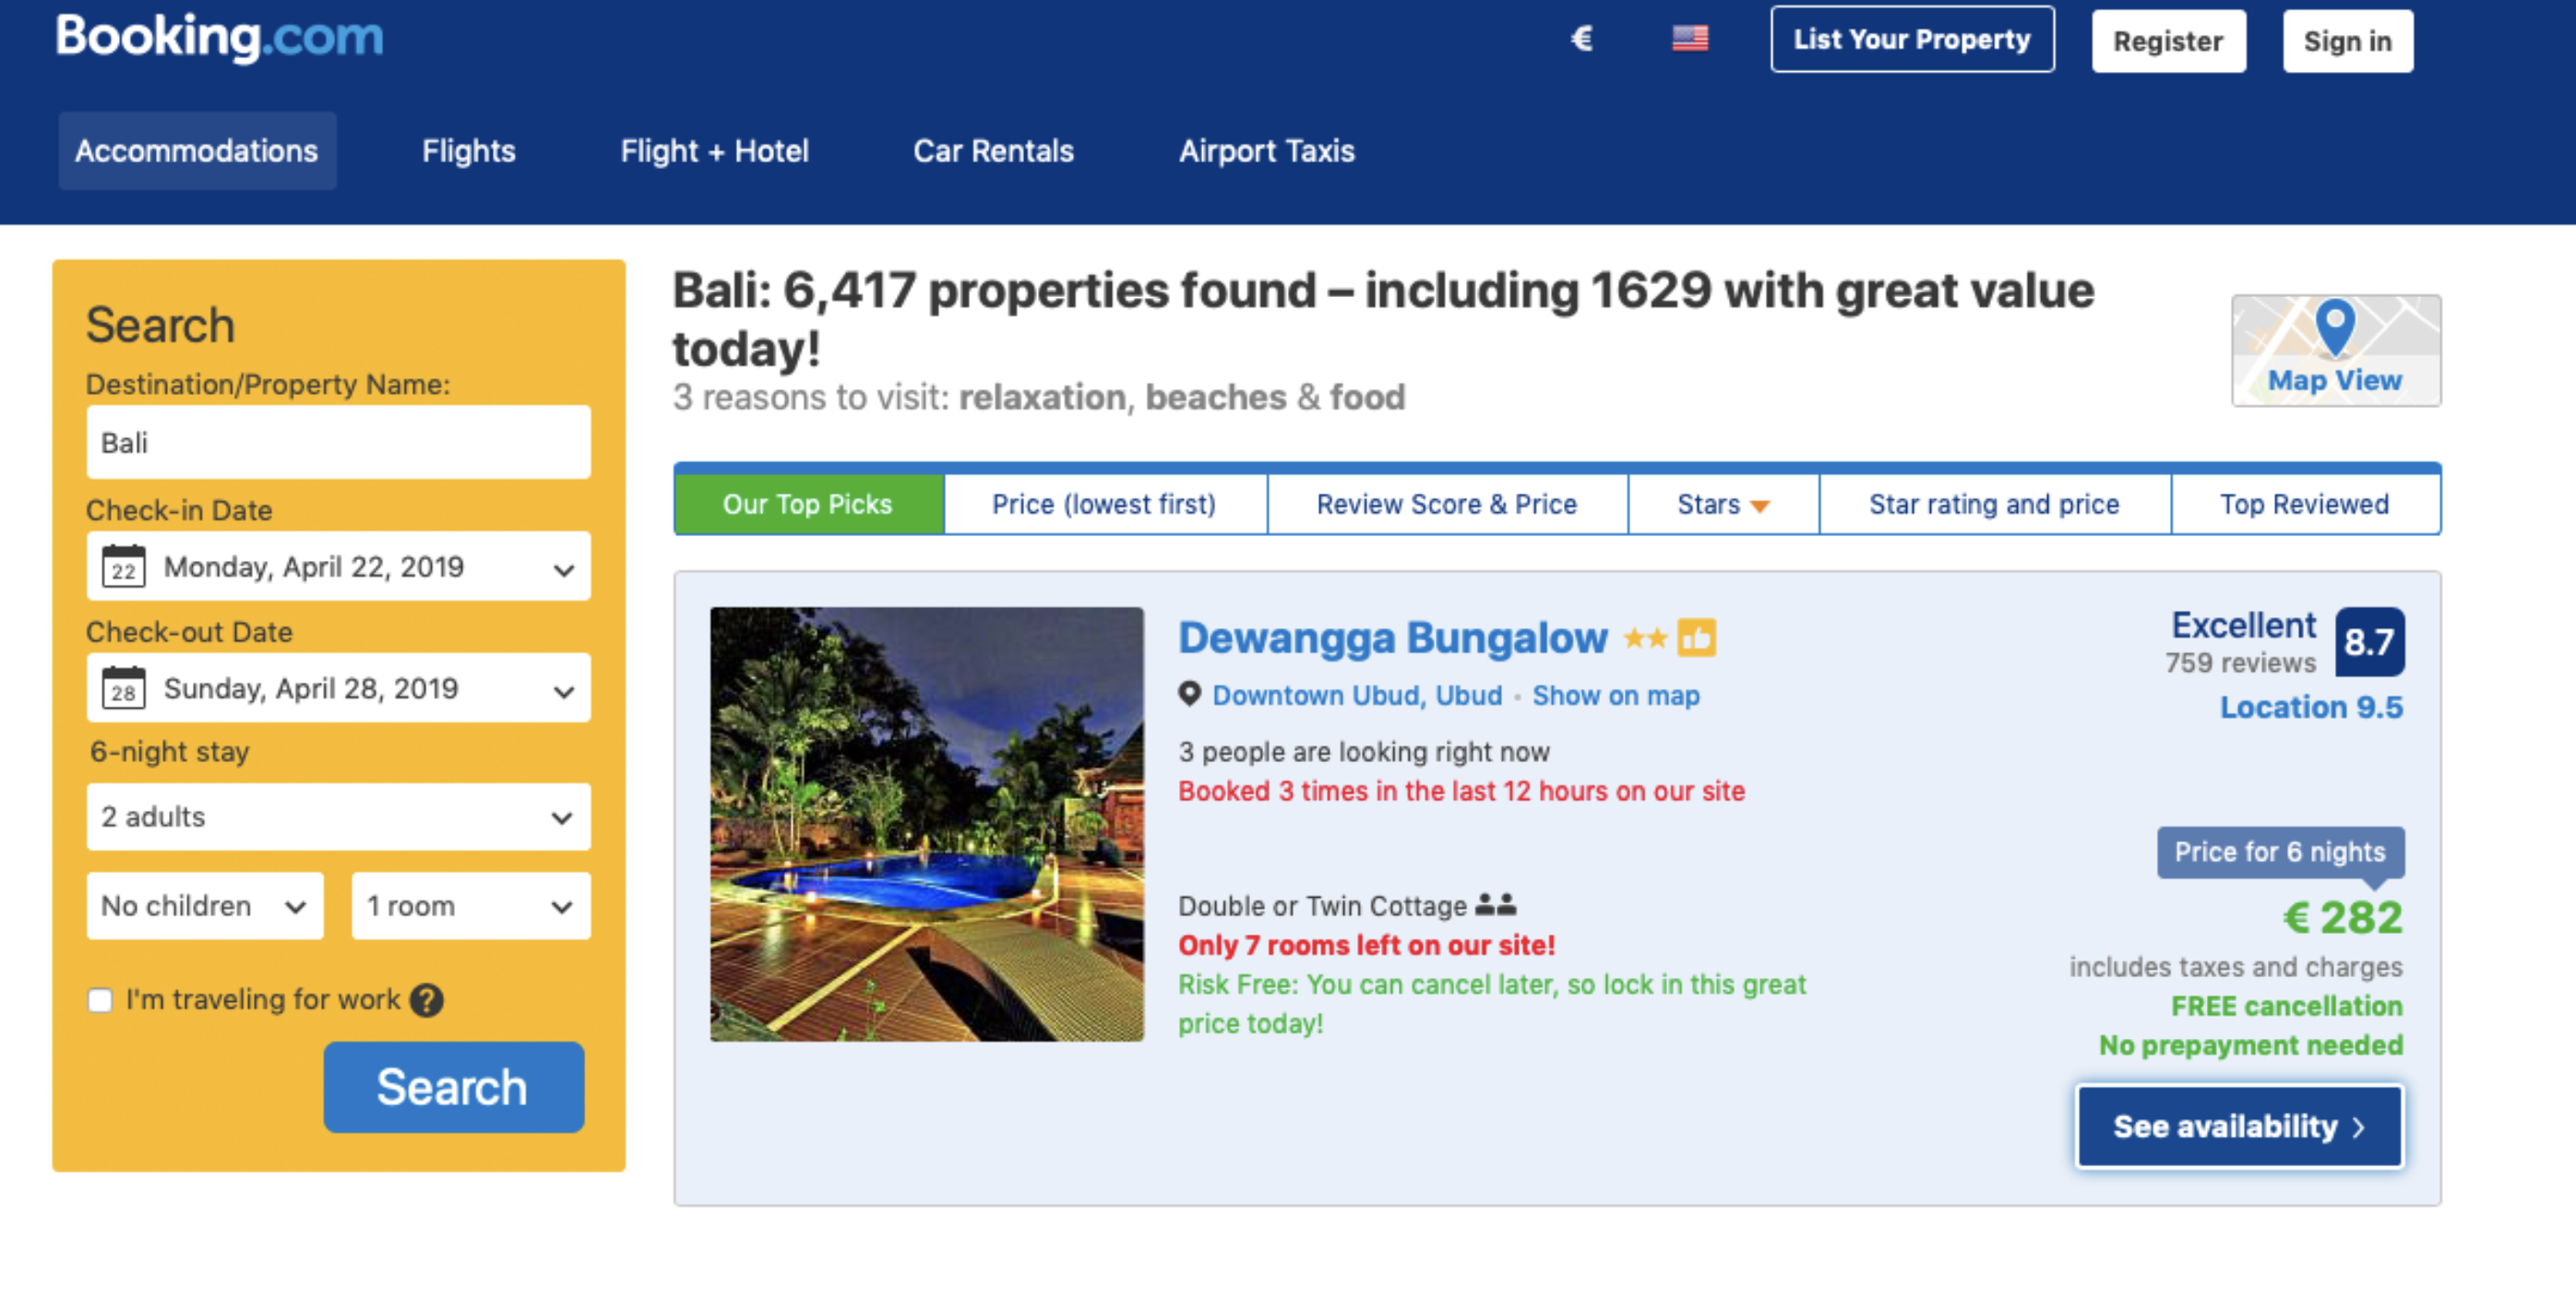
\includegraphics[width=1.0\textwidth]{booking-nudge.png}
    \caption{Digital nudging example - booking.com}
    \label{fig:booking}
\end{figure}

\newpage

%TODO Update graphic
\begin{figure}[h]
    \centering
    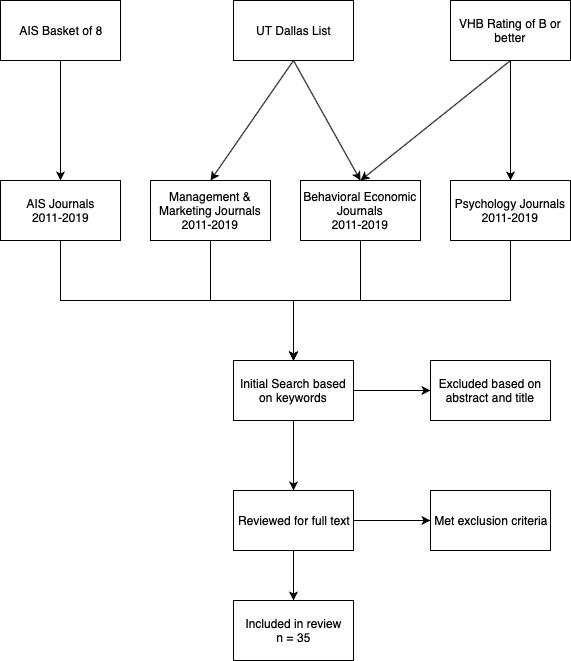
\includegraphics[width=1.0\textwidth]{method.png}
    \caption{Information flow of the screening process}
    \label{fig:method}
\end{figure}

\newpage

\begin{table}[h!]
\small
\centering
\begin{tabular}{l|l|p{9cm}|l}
 & \textbf{Library / Source} & \textbf{Journal} & \textbf{VHB Rating} \\ \hline
1 & AIS (Basket of 8) & European Journal of Information Systems & A \\ \hline
2 & AIS (Basket of 8) & Information Systems Journal & A \\ \hline
3 & AIS (Basket of 8) & Information Systems Research & A+ \\ \hline
4 & AIS (Basket of 8) & Journal of AIS & A \\ \hline
5 & AIS (Basket of 8) & Journal of Information Technology & A \\ \hline
6 & AIS (Basket of 8) & Journal of MIS & A \\ \hline
7 & AIS (Basket of 8) & Journal of Strategic Information systems & A \\ \hline
8 & AIS (Basket of 8) & MIS Quaterly & A+ \\ \hline
9 & UT Dallas & Journal on Computing & A \\ \hline
10 & UT Dallas & Journal of Consumer Research & A+ \\ \hline
11 & UT Dallas & Journal of Marketing & A+ \\ \hline
12 & UT Dallas & Journal of Marketing Research & A+ \\ \hline
13 & UT Dallas & Marketing Science & A+ \\ \hline
14 & UT Dallas & Management Science & A+ \\ \hline
15 & UT Dallas & Operations Research & A+ \\ \hline
16 & UT Dallas & Academy of Management Journal & A+ \\ \hline
17 & UT Dallas & Academy of Management Review & A+ \\ \hline
18 & UT Dallas & Journal of International Business Studies & A \\ \hline
19 & UT Dallas & Strategic Management Journal & A \\ \hline
20 & VHB & Journal of Behavioral Decision Making & B \\ \hline
21 & VHB & Journal of Behavioral and Experimental Economics & B \\ \hline
22 & VHB & Journal of Applied Behavioral Science & B \\ \hline
23 & VHB & Organizational Behavior and Human Decision Processes & A \\ \hline
24 & VHB & Applied Psychology & B \\ \hline
25 & VHB & European Journal of Work \& Organizational Psychology & B \\ \hline
26 & VHB & Journal of Applied Psychology & A \\ \hline
27 & VHB & Journal of Business and Psychology & B \\ \hline
28 & VHB & Journal of Consumer Psychology & A \\ \hline
29 & VHB & Journal of Economic Psychology & B \\ \hline
30 & VHB & Psychology \& Marketing & B \\ \hline
31 & AIS Conferences & Proceedings of the International Conference on Information Systems (ICIS) & A \\ \hline
32 & AIS Conferences & Proceedings of the European Conference on Information Systems (ECIS) & B \\
\end{tabular}
\caption{List of inspected journals}
\label{table:journals}
\end{table}

\newpage

%TODO Update figure
\begin{figure}[h!]
    \centering
    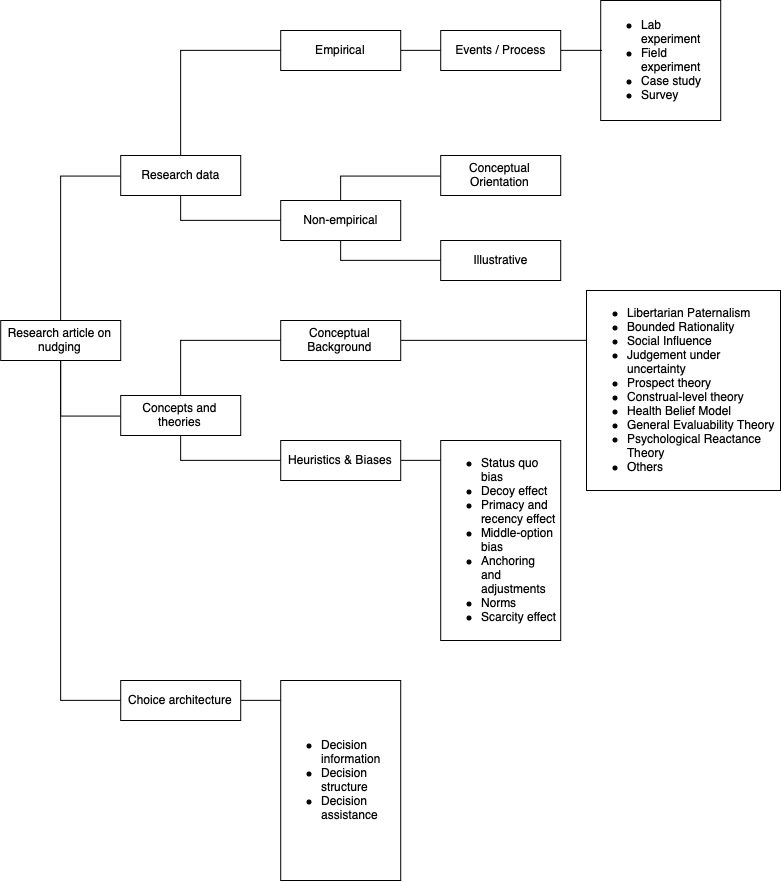
\includegraphics[width=1.0\textwidth]{analysis-2.png}
    \caption{Classification of findings-detailed}
    \label{fig:analysis-detail}
\end{figure}

\newpage

\begin{table}[h!]
\centering
\begin{tabular}{|l|l|}
\hline
\textbf{Domain} & \textbf{Coding} \\ \hline
Consumer Choice & CCH \\ \hline
Education & EDU \\ \hline
Finance & FIN \\ \hline
Health & HEA \\ \hline
Prosocial Behavior & PSB \\ \hline
Sustainability & SUS \\ \hline
Transportation & TRA \\ \hline
Security \& Privacy & SCP \\ \hline
Government & GOV \\ \hline
Other & MISC \\ \hline
\end{tabular}
\caption{List of domain codings}
\label{table:domain-coding}
\end{table}

\newpage


\newpage

%%%%%%%%%%%%%%%%%%%%%%%%%%%%%%%%%%%%%%%%%%%%%%%%%%%%%%%%%%%%%%%%%%%%%%%%%%%%%%%%%%%%%%%%%%%
% "Affidavit" Section
%%%%%%%%%%%%%%%%%%%%%%%%%%%%%%%%%%%%%%%%%%%%%%%%%%%%%%%%%%%%%%%%%%%%%%%%%%%%%%%%%%%%%%%%%%%

\sectionunnumbered{Affidavit} 
{I hereby declare that I have developed and written the enclosed seminar thesis entirely on my own and have not used outside sources without declaration in the text. Any concepts or quotations applicable to these sources are clearly attributed to them.\par}
\vspace{0.7cm}
{This seminar thesis has not been submitted in the same or substantially similar version, not even in part, to any other authority for grading and has not been published elsewhere. I am aware of the fact that a misstatement may have serious legal consequences.\par}
\vspace{0.7cm}

Mannheim,  \titledate\today %uncomment this line use date of today automatically
% Mannheim, 12. March 2019

\vspace{1.4cm}
Marvin Messenzehl


\end{document}